\chapter{SYSTEM DESIGN AND IMPLEMENTATION}

This chapter describes the implementation of the system which consists of two subsystems: A social media website and an analysis server. In \textit{Requirement analysis and System overview} subsection, everything is briefly described as a whole. In three last sections, structure and details of two subsystems and the database are defined more comprehensively.

\section{Requirement analysis and system overview}
\subsection{Requirement analysis}
\subsubsection{Functional Requirement}
\subsubsection{Non-functional Requirement}
\subsubsection{Use Cases}

\subsection{System overview}
Figure \ref{chap3:system_overview_basic} shows a concise overview of how the system operates. Users interact with the website through front-end. The input of users can come in the form of images, videos or label contribution. Back-end receives input and stores in the database. Concurrently, inputs are sent to analysis server . Outputs from analysis server are sent back to back-end and then stored in database. The back-end is also responsible for obtaining appropriate contents from the database to display to users through front-end.

\begin{center}
    \begin{figure}[H]
    \centering
    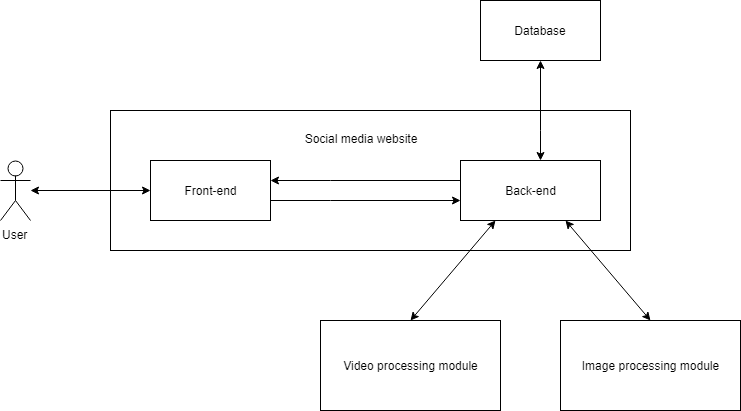
\includegraphics[width=1\columnwidth]{images/chap3/system_overview_basic.png}
    \caption{An overview of the system}
    \label{chap3:system_overview_basic}
    \end{figure}
\end{center}
\section{Database}
The project database divides into two different parts: \textbf{Cloud storage} for visual data such as image/video and a \textbf{NoSQL database} for other information. The primary target is to reduce website loading time. Let take an example, if files are stored directly on the back-end server. When many users request a file simultaneously, the server with limited bandwidth will cause delay. “53\% of mobile site visitors leave a page that takes longer than three seconds to load” – \href{https://think.storage.googleapis.com/docs/mobile-page-speed-new-industry-benchmarks.pdf}{Google}. If these files stored on cloud storage, the client will be served by the cloud storage provider, which has higher availability.
\subsection{Cloud storage}

\subsection{NoSQL database}
NoSQL databases were created in response to the limitations of traditional relational database technology. When compared against relational databases, NoSQL databases are more scalable and provide superior performance, and their data model addresses several shortcomings of the the relational model.

The advantages of NoSQL include being able to handle:

Large volumes of structured, semi-structured, and unstructured data
Agile sprints, quick iteration, and frequent code pushes
Object-oriented programming that is easy to use and flexible
Efficient, scale-out architecture instead of expensive, monolithic architecture
Hence, \textbf{MongoDB} is used to implement the database in this project
\subsubsection{Database overview}
Figure \ref{chap4:database_overview} displays the structure of the database which includes collections and relationships between them.
There are a total of 8 collections in the database: User, Visual data, Location, Notification, Person, Post, Record, Role. 
\begin{center}
    \begin{figure}[H]
    \centering
    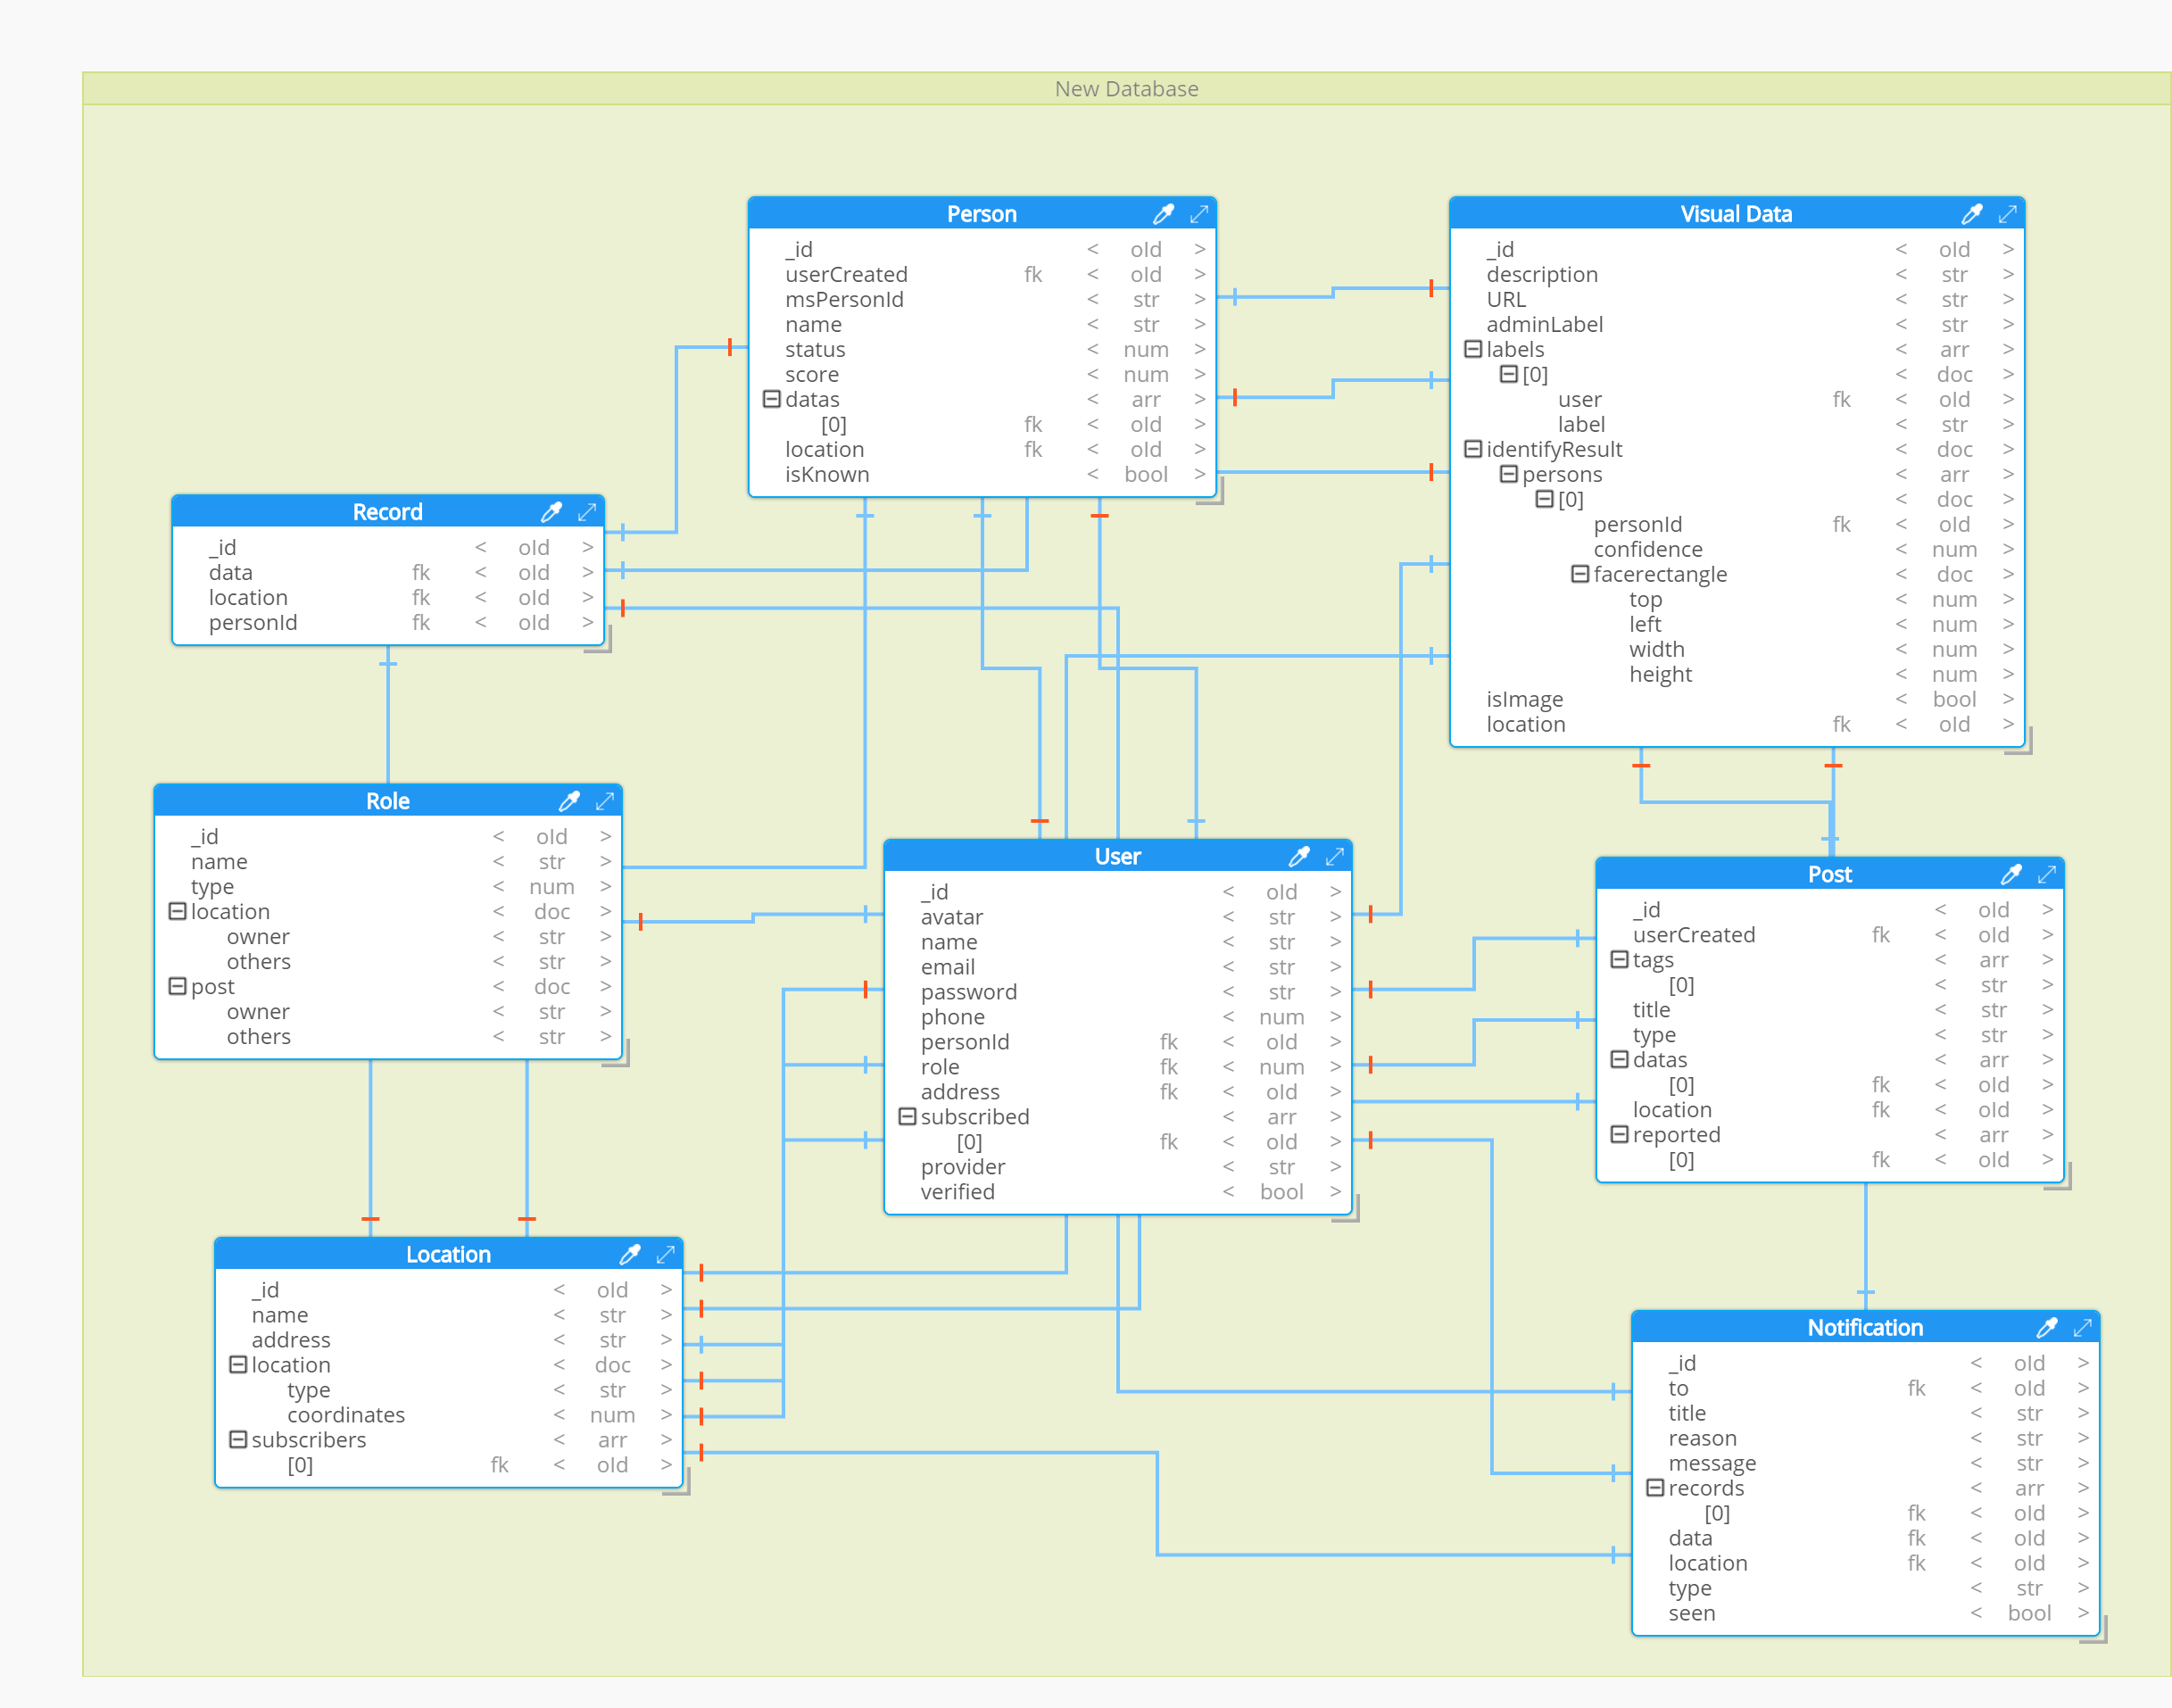
\includegraphics[width=1\columnwidth]{images/chap4/Model.png}
    \caption{An overview of the database}
    \label{chap4:database_overview}
    \end{figure}
\end{center}
\cleardoublepage
\subsubsection{Collections}
\textbf{User}
\begin{center}
    \begin{figure}[H]
    \centering
    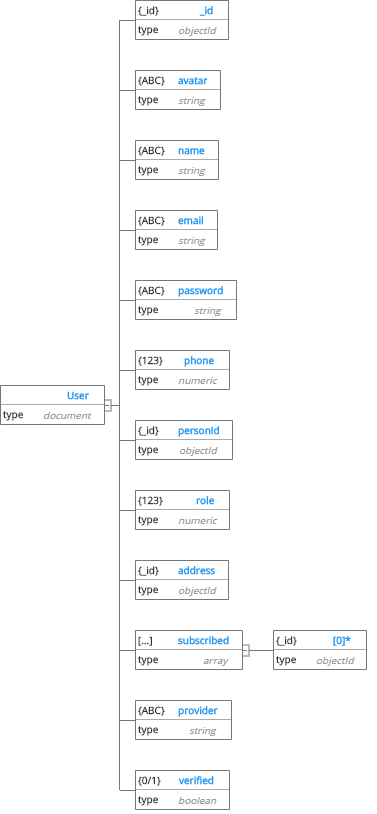
\includegraphics[width=0.5\columnwidth]{images/chap4/User.png}
    \caption{User collection}
    \end{figure}
\end{center}
\cleardoublepage
\textbf{Visual data}
\begin{center}
    \begin{figure}[H]
    \centering
    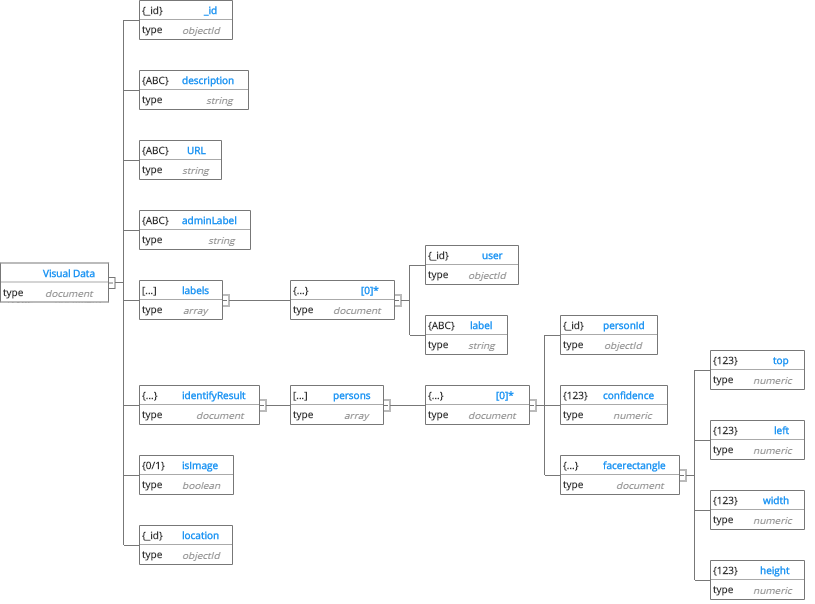
\includegraphics[width=1\columnwidth]{images/chap4/Visual.png}
    \caption{Visual Data collection}
    \end{figure}
\end{center}
\cleardoublepage
\textbf{Location}
\begin{center}
    \begin{figure}[H]
    \centering
    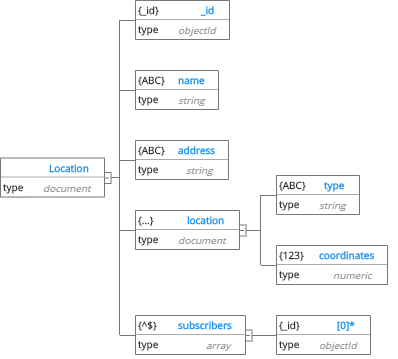
\includegraphics[width=1\columnwidth]{images/chap4/Location.png}
    \caption{Location collection}
    \end{figure}
\end{center}
\cleardoublepage
\textbf{Notification}
\begin{center}
    \begin{figure}[H]
    \centering
    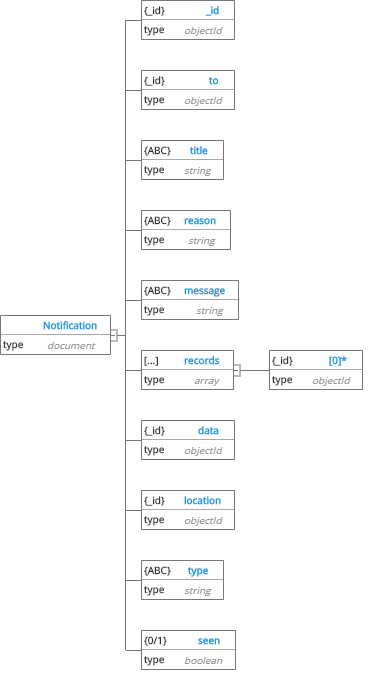
\includegraphics[width=0.7\columnwidth]{images/chap4/Notification.png}
    \caption{Notification collection}
    \end{figure}
\end{center}
\cleardoublepage
\textbf{Person}
\begin{center}
    \begin{figure}[H]
    \centering
    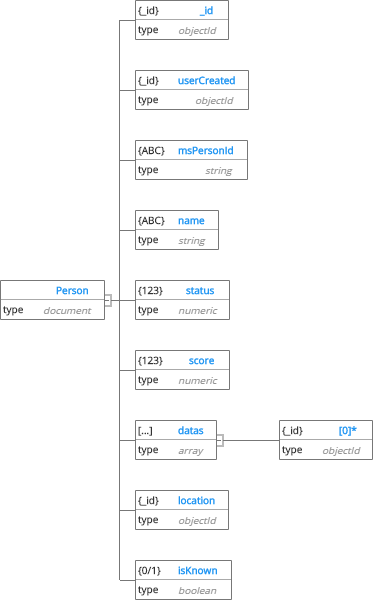
\includegraphics[width=0.7\columnwidth]{images/chap4/Person.png}
    \caption{Person collection}
    \end{figure}
\end{center}
\cleardoublepage
\textbf{Post}
\begin{center}
    \begin{figure}[H]
    \centering
    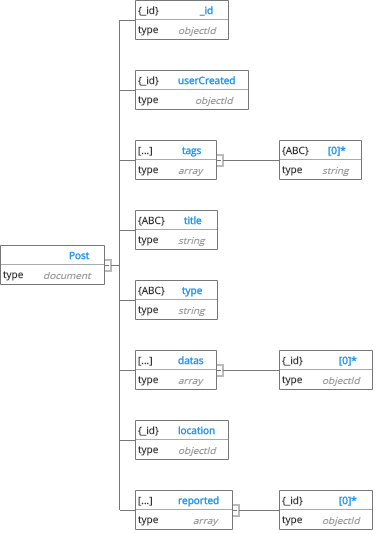
\includegraphics[width=0.7\columnwidth]{images/chap4/Post.png}
    \caption{Post collection}
    \end{figure}
\end{center}
\cleardoublepage
\textbf{Record}
\begin{center}
    \begin{figure}[H]
    \centering
    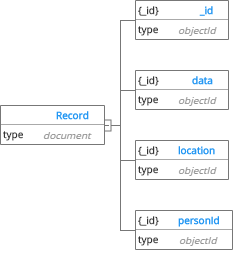
\includegraphics[width=0.7\columnwidth]{images/chap4/Record.png}
    \caption{Record collection}
    \end{figure}
\end{center}
\cleardoublepage
\textbf{Role}
\begin{center}
    \begin{figure}[H]
    \centering
    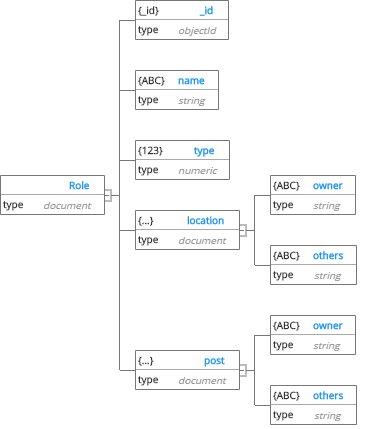
\includegraphics[width=0.7\columnwidth]{images/chap4/Role.png}
    \caption{Role collection}
    \end{figure}
\end{center}
\cleardoublepage
\subsubsection{Relationships}
\begin{table}[H]
\begin{tabular}{|l|l|}
\hline
\textbf{Children field}                                      & \textbf{Parent field}     \\ \hline
Location.subscribers.{[}0{]}                        & User.\_id        \\ \hline
Notification.to                                     & User.\_id        \\ \hline
Notification.records.{[}0{]}                        & Record.\_id      \\ \hline
Notification.data                                   & Visual Data.\_id \\ \hline
Notification.location                               & Location.\_id    \\ \hline
Person.userCreated                                  & User.\_id        \\ \hline
Person.datas.{[}0{]}                                & Visual Data.\_id \\ \hline
Person.location                                     & Location.\_id    \\ \hline
Post.userCreated                                    & User.\_id        \\ \hline
Post.datas.{[}0{]}                                  & Visual Data.\_id \\ \hline
Post.location                                       & Location.\_id    \\ \hline
Post.reported.{[}0{]}                               & User.\_id        \\ \hline
Record.data                                         & Visual data.\_id \\ \hline
Record.location                                     & Location.\_id    \\ \hline
Record.personId                                     & Person.\_id      \\ \hline
User.personId                                       & Person.\_id      \\ \hline
User.address                                        & Location.\_id    \\ \hline
User.subscribed.{[}0{]}                             & Location.\_id    \\ \hline
Visual Data.labels.{[}0{]}.user                     & User.\_id        \\ \hline
Visual Data.identifyResult.persons.{[}0{]}.personId & Person.\_id      \\ \hline
Visual Data.location                                & Location.\_id    \\ \hline
User.role                                           & Role.type        \\ \hline
\end{tabular}
\end{table}
\cleardoublepage
Example:
\begin{table}[H]
\begin{tabular}{|l|l|}
\hline
Children field               & Parent field \\ \hline
Location.subscribers.{[}0{]} & User.\_id    \\ \hline
\end{tabular}
\end{table}
The element of the field \textit{subscribers}(array) of collection \textbf{Location} references field \textit{\_id} of collection \textbf{User}.
\section{Social media website}
\subsection{Front-end}
\subsection{Back-end}
\section{Analysis server}
The project requires two systems for analysis: A face recognition system and a video classifier system. The facial recognition system takes pictures of human faces as input and returns their identification. The video classifier system analyzes videos to find out actions in them. The remaining of this section describes in detail about the two analysis system.
\subsection{Face recognition module}
\subsection{Video classifier module}
Video classifying is not a new task in the field of Deep learning.
	
\section{Technologies}
\subsection{Node.js and npm}
Node.js (Node) is a JavaScript runtime built on Chrome's V8 JavaScript engine (cite). Node supports executing JavaScript on server-side. Ryan Dahl was created Node.js in 2009. Node.js Foundation is in charge of the development of Node.js. After nine years since its release, the latest LTS version of Node.js is 10.14.2 (includes npm 6.4.1). “Node.js operates on a single thread, using non-blocking I/O calls, allowing it to support tens of thousands (cite) of concurrent connections held in the event loop.” Although JavaScript is single-threaded, thanks to the Event loop, Node.js can implement asynchronous I/O operations. The Event loop will transfer operations to the system kernel. “Since most modern kernels are multi-threaded, they can handle multiple operations executing in the background. When one of these operations completes, the kernel tells Node.js so that the appropriate callback may be added to the poll queue to executed eventually”. By utilizes non-blocking I/O, Node.js skips the waiting time for I/O calls, which is much higher than processing time.